\section{RAVEN Theory by way of Examples: Reduced Order Modeling}
The development of high-fidelity codes, for thermal-hydraulic systems 
and integrated multi-physics, has undergone a significant acceleration 
in the last years. Multi-physics codes involve simulations that treat 
multiple physical models or multiple simultaneous physical phenomena, 
in a integrated solving environment. Multi-physics typically involves 
solving coupled systems of partial differential equations, generally 
characterized by several different geometrical and time scales. 
\\The new multi-physics codes are characterized by remarkable 
improvements 
in the approximation of physics (high approximation order and reduced 
use of empirical correlations). This greater fidelity is generally 
accompanied by a greater computational effort (calculation time 
increased). This peculiarity is an 
obstacle in the application of  computational techniques of 
quantification of uncertainty and risk associated with the operation of 
particular industrial plant (for example, a nuclear reactor). 
\\As already reported, a solution to this problem is represented by the 
usage
of highly effective sampling strategies. Sometimes also these 
approaches is not enough
in order to perform a comprehensive UQ and PRA analysis. In these 
cases the help of reduced order modeling is essential.
\\RAVEN has support of several different reduced order model (ROM), 
such as:
\begin{enumerate}
  \item \textit{Nearest Neighbors approaches};
  \item \textit{Support Vector Machines};
  \item \textit{Inverse Weight regressors};
  \item \textit{Spline regressors }, etc.
\end{enumerate}
In this section only few of them are going to be analyzed, explaining the theory behind it
by way of applied RAVEN examples.


As briefly and previously mentioned, a ROM, also called a surrogate 
model, is a mathematical representation of a system, used to predict 
a selected FOM of a physical system.
\\The ``training'' is a process that, sampling the physical model 
represented by the high fidelity simulator (e.g., RELAP 7, RELAP5 
3D, PHISICS, etc.), is aimed to improve the prediction capability 
(ability to predict the status of the system given a realization of the 
uncertain domain) of the ROM. 
\begin{figure}[h!]
  \centering
  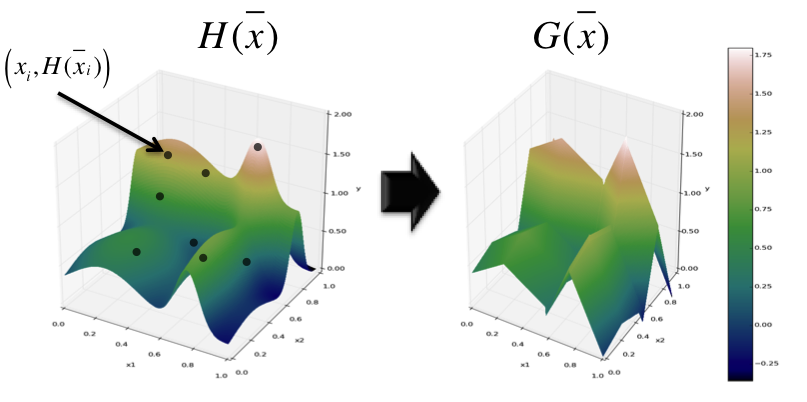
\includegraphics[width=1.0\textwidth]  {pics/ROMexampleOfPhysicalSystem.png}
  \caption{Example of reduced order model representation of physical system (regression).}
  \label{fig:ROMexampleOfPhysicalSystem}
\end{figure}
\\Two characteristics of these models 
are generally assumed (even if exceptions are possible):
\begin{enumerate}
  \item The higher the number of realizations in the training sets, the 
higher the accuracy of the prediction performed by the ROM is. This 
statement is true for most of the cases although some ROMs might be 
subject to the over-fitting issues. The over-fitting phenomenon is not 
analyzed in this thesis, since its occurrence highly depends on the 
algorithm type, and, hence, the problem needs to be analyzed for all 
the large number of ROM types available;
  \item The smaller the size of the input (uncertain) domain with 
  respect to the variability of the system response, the more likely the 
  ROM is able to represent the system response space.
\end{enumerate}

To provide a very simple idea of a ROM, assume that the final 
response space of a physical system is governed by the transfer 
function $H \left (  \overline{x}\right)$ (see 
\ref{chap:mathBackground}), which, from a practical point of 
view, represents the outcome of the system, based on the initial 
conditions  $\overline{x}$. Now, sample the domain of variability of the 
initial conditions $\overline{x}$ to create a 
set of $N$ realizations of the input and response space $ \left ( \left ( 
\overline{x}_{i}, H \left (  \overline{x}_{i}\right) \right), i=1,N \right)$, 
named ``training'' set. Based on the data set generated, it is possible 
to construct a mathematical representation $G\left ( \overline{x}:
\overline{x}_{i}\right)$ of the 
real system $H \left (  \overline{x}\right)$, which will approximate its 
response (see Figure~\ref{fig:ROMexampleOfPhysicalSystem}):
\begin{equation}
\label{eq:regressor}
G\left ( \overline{x} \right ):\overline{x}_{i} \rightarrow G\left ( \overline{x}_{i} \right ) \cong H\left ( \overline{x}_{i} \right )
\end{equation}
The ROMs reported above are generally named ``regressors'', among 
which all the most common data fitting algorithms are found (e.g., 
least square for construction of linear models).
\\An important class of ROMs for the work presented here after is the 
one containing the so called ``classifiers''. A classifier is a ROM that is 
capable of representing the system behavior from a binary point of 
view (e.g., event happened/not happened or failure/success). It is a 
model (set of equations) that identifies to which category an object 
belongs in the feature (input) space. Referring to the example that 
brought to Eq.~\ref{eq:regressor}, a classifier can be formally represented as follows (see 
Figure~\ref{fig:ROMClassifierExampleOfPhysicalSystem}):
\begin{figure}[h!]
  \centering
  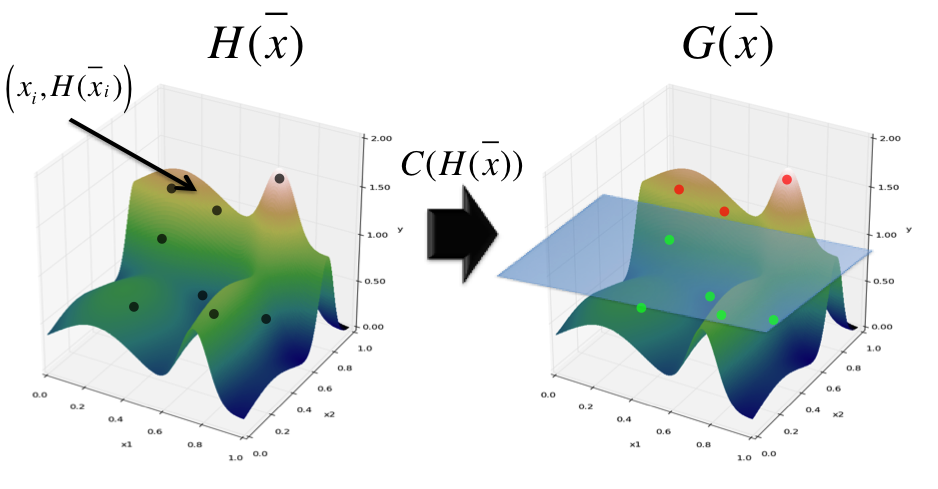
\includegraphics[width=1.0\textwidth]  {pics/ROMClassifierExampleOfPhysicalSystem.png}
  \caption{Example of reduced order model representation of physical system (classifier).}
  \label{fig:ROMClassifierExampleOfPhysicalSystem}
\end{figure}

\begin{equation}
\label{eq:classifier}
G\left ( \overline{x} \right ):\overline{x}_{i} \rightarrow G\left ( \overline{x}_{i} \right ) \cong 
C \left ( H\left ( \overline{x}_{i} \right ) \right )
\end{equation}

The function $C\left (  H\left ( \overline{x}_{i}  \right ) = \overline{\theta} 
\right ) $ is the so called ``goal'' function that is able to recast the 
response of the system $H\left ( \overline{x}_{i}  \right )$ into a binary 
form (e.g., failure/success). As an example, referring to 
Figure~\ref{fig:ROMClassifierExampleOfPhysicalSystem}, the 
``goal'' function would be:
\begin{equation}
\label{eq:goalFunctionClassifier}
C\left (   \overline{\theta}  \right ) = \left\{\begin{matrix}
1 & if \: \overline{\theta}>1.0 \\ 
0 &  if \: \overline{\theta} \leq 1.0
\end{matrix}\right.
\end{equation}
Hence, the ROM of type classifier $G\left (  \overline{x} \right )$  will operate in the space transformed through the ``goal''  function $C\left (   \overline{\theta}  \right )$. 
\\The classifiers and regressors can be categorized into two main classes:
\begin{itemize}
  \item Model based algorithms;
  \item Data based algorithms.
\end{itemize}
In the first class, the created ROM aims to approximate the response 
of the system as a function of the input parameters. These algorithms 
construct a functional representation of the system. Examples of such ROM type are support vector machines (SVMs), Kriging-based interpolators, discriminant based models, and polynomial chaos.
\\On the other side, data based algorithms do not build a response-
function-based ROM but classify or predict the response of the 
system from the neighborhood graph constructed from the training 
data, without any dependencies on a particular prediction model.
\\These algorithms directly build a neighborhood structure as the 
ROM (e.g., a relaxed Gabriel graph) on the initial training data. Examples of such ROM type are nearest neighbors and decision trees.

\subsection{Gaussian Process Models}
\label{sec:GPM}
Gaussian processes (GPs)~\cite{Rasmussen_GPM} are algorithms that extend multivariate Gaussian distributions to infinite dimensionality. A Gaussian process generates a data set located throughout some domain such that any finite subset of the range follows a multivariate Gaussian distribution. Now, the n observations in an arbitrary data set, $y={y_1,\ldots,y_n}$, can always be imagined as a single point sampled from some multivariate ($n$-variate) Gaussian distribution.
What relates one observation to another in such cases is just the covariance function, $k(x,x')$. A popular choice is the squared exponential:
\begin{equation}
k(x,x')=\sigma_{f}^{2}  exp \left [ \frac{-(x-x')^2}{2 l^2} \right ]
\end{equation}
where the maximum allowable covariance is defined as $\sigma_{f}^{2}$; this should be high for functions which cover a broad range on the y axis. If $x \simeq x'$, then $k(x,x')$ approach this maximum meaning $f(x)$ is very correlated to $f(x')$. On the other hand, if $x$ is very distant from $x'$, then $k(x,x' ) \simeq 0$, i.e. the two points cannot see each other. 
So, for example, during interpolation at new $x$ values, distant observations will have negligible effect. How much effect this separation has will depend on the length parameter $l$.
Each observation $y$ can be thought of as related to an underlying function $f(x)$ through a Gaussian noise model:
\begin{equation}
y=f(x)+N(0,\sigma_{n}^{2})
\end{equation}
The new kernel function can be written as:
\begin{equation}
k(x,x')=\sigma_{f}^{2}  exp \left [ \frac{-(x-x')^2}{2 l^2} \right ] + \sigma_{n}^{2} \delta(x,x')
\end{equation}
So given $n$ observations $y$, the objective is to predict the value $y_*$ at the new point $x_*$. This process is performed by following this sequence of steps:
\begin{enumerate}
\item Calculate three matrices:
\begin{equation}
K=\begin{bmatrix}
k(x_1,x_1) &  \ldots & k(x_1,x_n)\\ 
\vdots  & \ddots &\vdots  \\ 
k(x_n,x_1) &  \ldots & k(x_n,x_n)
\end{bmatrix}
\end{equation}
\begin{equation}
K_*= \begin{bmatrix}
k(x_*,x_1) & \ldots & k(x_*,x_n)
\end{bmatrix}
\end{equation}
\begin{equation}
K_{**}=k(x_*,x_*)
\end{equation}
\item The basic assumption of GPM is that:
\begin{equation}
\begin{bmatrix}
y\\
y_* 
\end{bmatrix}
=\mathcal{N}(0,\begin{bmatrix}
K & K_{*}^{T}\\ 
K_* & K_{**}
\end{bmatrix})
\end{equation}
\item The estimate $\bar{y_*} $ for $y_*$ is the mean of this distribution
\begin{equation}
\bar{y_*}=K_* K^{-1}y
\end{equation}
\item The uncertainty associated to the estimate $\bar{y_*} $ can be expressed in terms of variance of  $y_*$:
\begin{equation}
var(y_*)=K_{**}-k_* K^{-1} K_{*}^{T}
\end{equation}
\end{enumerate}

\subsection{Support Vector Machines}
\label{sec:SVM}
The Support Vector Machine~\cite{SVM_Burges} classifier is a methodology that aims to determine the optimal separation hyperplane between data sets having different labels.
The training data consist of $N$ data points $(x_i,y_i)$ $i=1,\ldots,N$ where $x_i \in \mathbb{R}^M$ and $y_i \in {-1,1}$.
Assuming a linear property of the hyperplane  then its definition is:
\begin{equation}
\left \{ x: f(x)=x^T\beta+\beta_0=0 \right \}
\end{equation}
where $\beta$ is a unit vector. 

The SVM parameters $\beta$ and $\beta_0$  are determined by solving this optimization problem:
\begin{equation}
\left\{\begin{matrix}
\underset{\beta,\beta_0}{min} \left \| \beta \right \|\\ 
\text{subject to } y_i(x_{i}^{T}\beta+\beta_0)\geq 1 , \quad i=1,\dots,N
\end{matrix}\right.
\end{equation}

Once the SVM parameters $\beta$ and $\beta_0$ are determined then the classification of a new point $\bar{x}$ is given by:
\begin{equation}
G(\bar{x})=sign(\bar{x}^T\beta+\beta_0)
\end{equation}


\subsection{KNN Classifier and KNR Regressor}
\label{sec:KNN_KNR}
The K Nearest Neighbor algorithm~\cite{altman_KNN} (KNN) is a non-parametric method used for both regression and classification. The only input parameter is the variable $K$ which indicates the number of neighbors to be considered in the classification/regression process. The special case where the class is predicted to be the class of the closest training sample (i.e. when $K = 1$) is called the nearest neighbor algorithm. In binary (two class) classification problems, it is helpful to choose k to be an odd number as this avoids tied votes. The output depends on whether KNN is used for classification or regression:
\begin{itemize}
\item In KNN classification, the output is a class membership. An object is classified by a majority vote of its neighbors, with the object being assigned to the class most common among its $K$ nearest neighbors ($K$ is a positive integer, typically small). If $K = 1$, then the object is simply assigned to the class of that single nearest neighbor.
\item In KNN regression, the output is the property value for the object. This value is the average of the values of its $K$ nearest neighbors.
\end{itemize}
Both for classification and regression, it can be useful to assign weight to the contributions of the neighbors, so that the nearer neighbors contribute more to the average than the more distant ones. For example, a common weighting scheme consists in giving each neighbor a weight of $1/d$, where $d$ is the distance to the neighbor.



\section{Multi-Dimensional Interpolation}
\label{sec:MD_interp}

This section covers the methods that have been implemented in the CROW statistical library:
\begin{itemize}
\item Sheppard Method (see Section~\ref{sec:sheppard})
\item Multi-Dimensional Spline method (see Section~\ref{sec:ND_spline})
\end{itemize}

These two methods are interpolation methods that can be used in any dimension.
In RAVEN they are employed in two major applications:
\begin{enumerate}
\item Reduced Order Models
\item Multi-dimensional distributions
\end{enumerate}
For both applications, given a set of $N$ data points $ (x_i,u_i )$  $i=1,\ldots,N$ where $x_i$ are the coordinate in the input space $D \subset \mathbb{R}^M$ and $u_i \in \mathbb{R}$ is the outcome, the methods predicts the outcome $\tilde{u}$ for a new coordinate $\tilde{x}\in \mathbb{R}^n$.


\subsection{Shepard Method}
\label{sec:shepard}
The Shepard interpolator~\cite{Shepard} isalso know as Inverse Distance Weighting (IDW) interpolator. 
The starting point is a set of $N$ data points $ (x_i,u_i )$ for $i=1,\ldots,N$. 
The Inverse-Weight interpolator can be represented as a function $f_{IDW}(x)$ that, given a new coordinate in the input space $x$, generates a prediction on $u$ such that 
\begin{equation}
u:x \in \mathbb{R}^M \rightarrow f_{IDW}(x) \in \mathbb{R}
\end{equation}
based on the distance $d(x,x_i)$ in the euclidean space between $x$ and $x_i$.

Such prediction $u=f_{IDW}(x)$ is performed by summing all data points $x_i$ $i=1,\ldots,N$ weighted by a weighting parameter $w_i (x)$ as follows:
\begin{equation}
f_{IDW}(x) = 
\left\{
\begin{matrix}
\sum_{i=1}^{N} w(x_i) u_i &  \text{if } d(x,x_i) \neq 0 \\
 u_i &  \text{if } d(x,x_i) = 0
\end{matrix}\right.
\end{equation}
where
\begin{equation}
w(x_i) =\frac{w_i}{\sum_{i=1}^{N} w_i}
\end{equation}
and
\begin{equation}
w_i = \left ( \frac{1}{d(x,x_i)} \right )^p
\end{equation}
Large values of $p$ assign greater weight $w_i$ to data points $x_i$ closest to $x$, with the result turning into a mosaic of tiles (i.e., Voronoi diagram) with nearly constant interpolated value.

\subsection{Multi-Dimensional Spline}
\label{sec:ND_spline}
The Multi-Dimensional Spline (MDS)~\cite{MD_spline} is a method which requires the sampled points $x_i$ to be lying in multi-dimensional cartesian grid.
A generic grid $\Delta_m$ for each dimension $m$ will be indicated as follows:
\begin{equation}
\Delta_m = \{x_{0_m},x_{1_m},\ldots,x_{p_m}\} \text{ for } m=1,\ldots,M
\end{equation}
This methods construct a $M$-dimensional cubic spline so that, given a coordinate in the input space $x=(x_1,x_2,\ldots,x_M)$, generates a prediction on $u$ such that 
\begin{equation}
u:x \in \mathbb{R}^M \rightarrow f_{MDS}(x) \in \mathbb{R}
\end{equation}
where
\begin{equation}
f_{MDS}(x)=\sum_{i_1=1}^{p_1+3} \sum_{i_2=1}^{p_2+3} \ldots \sum_{i_M=1}^{p_M+3} c_{i_1,i_2,\ldots,i_p} \prod_{m=1}^{M} u_{i_j} (x_m)
\end{equation}
where 
\begin{equation}
u_{i_j} (x_m) = \Phi\left ( \frac{x_m-x_{0_m}}{h_j}+2-i_j  \right )
\end{equation}

The cubic kernel $\Phi(t)$ is defined as:
\begin{equation}
\Phi(t) = \left\{\begin{matrix}
(2-\left | t \right |)^3 & 1\leq \left | t \right |\leq 2 \\
4-6\left | t \right |^2+3\left | t \right |^3 & \left | t \right |\leq 1\\ 
0 & \text{elsewhere}
\end{matrix}\right.
\end{equation}

The set of $\prod_{m=1}^{M}(p_m+3)$ coefficients $c_{i_1,i_2,\ldots,i_p}$  is determined when the interpolator is initialized.




%%%%%%%%%%%%%%%%%%%%%%%%%%%%%%%%
%%%%%%%%  Limit Surface Search %%%%%%%% 
%%%%%%%%%%%%%%%%%%%%%%%%%%%%%%%%
\subsection{Limit Surface Search Method}
\label{sub:LS}
sssssss


%%%%%%%%%%%%%%%%
\subsubsection{Limit Surface Search sampling through RAVEN}
\label{subsub:LSsamplingExample}
The goals of this section are about learning how to:
 \begin{enumerate}
   \item Set up a Limit Surface Search sampling for efficiently perturb a driven code;
   \item Use the Limit Surface Integral Post-processor for computing the probability of failure of the system subject to the same 
   ``goal'' function;
   \item Plot the obtained Limit Surface.
\end{enumerate}  
In order to accomplish these tasks, the following RAVEN \textbf{Entities} (XML blocks in the input files) need to be defined:
\begin{enumerate}
   \item \textbf{\textit{RunInfo}}:
\begin{lstlisting}[style=XML,morekeywords={arg,extension,pauseAtEnd,overwrite}]
  <RunInfo>
    <JobName>LSsearch</JobName>
    <Sequence>
      sample,computeLSintegral,writeHistories
    </Sequence>
    <WorkingDir>LSsearch</WorkingDir>
    <batchSize>8</batchSize>
  </RunInfo>
\end{lstlisting}   
   As reported in section~\ref{sub:EntitiesAndFlow}, the \textit{RunInfo} \textbf{Entity} is intended to set up the analysis 
   that the user wants to perform. In this specific case, three steps (\xmlNode{Sequence}) are going to be sequentially run 
   using 8 processors (\xmlNode{batchSize}). 
   \item \textbf{\textit{Files}}:
\begin{lstlisting}[style=XML,morekeywords={arg,extension,pauseAtEnd,overwrite}]
  <Files>
    <Input name="referenceInput.xml" type="input">referenceInput.xml</Input>
    <Input name="LSintegral.csv" type="">LSintegral.csv</Input>
  </Files>
\end{lstlisting}
   Since the driven code uses a single input file, in this section the original input is placed. As detailed in the user manual
   the attribute  \xmlAttr{name} represents the alias that is going to be 
   used in all the other input blocks in order to refer to this file. 
   \\In addition the output file used in \xmlNode{Sequence} 
   \textit{computeLSintegral} is here inputted.
   \item \textbf{\textit{Models}}:
\begin{lstlisting}[style=XML,morekeywords={arg,extension,pauseAtEnd,overwrite}]
  <Models>
    <Code name="testModel" subType="GenericCode">
      <executable>
      ../physicalCode/analyticalbateman/AnalyticalDplMain.py
      </executable>
      <clargs arg="python" type="prepend"/>
      <clargs arg="" extension=".xml" type="input"/>
      <clargs arg="" extension=".csv" type="output"/>
      <prepend>python</prepend>
    </Code>
    <ROM name="AccelerationROM" subType="SciKitLearn">
      <Features>sigma-A,decay-A</Features>
      <Target>goalFunction</Target>
      <SKLtype>neighbors|KNeighborsClassifier</SKLtype>
      <n_neighbors>1</n_neighbors>
    </ROM>
    <PostProcessor name="integralLS" subType="LimitSurfaceIntegral">
      <tolerance>0.001</tolerance>
      <integralType>MonteCarlo</integralType>
      <seed>20021986</seed>
      <target>goalFunction</target>
      <variable name="sigma-A">
        <distribution>sigmaA</distribution>
      </variable>
      <variable name="decay-A">
        <distribution>decayConstantA</distribution>
      </variable>
    </PostProcessor>
  </Models>
\end{lstlisting}
 As mentioned above, the goal of this example is the employment of 
 an efficient sampling strategy, having as goal the determination of the
 failure of a system.
 \\Indeed, in addition to the previously explained Code 
 model,
 the ROM of type \textit{SciKitLearn} is here specified. The ROM will be
 used in the adaptive sampling strategy \textit{LimitSurfaceSearch} in
 order to accelerate the convergence of the method. As it can be seen,
 a nearest neighbor classifier is used, targeting only two uncertainties 
 $sigma-A and decay-A$.
 \\ For the computation of the probability of failure (see the following), a 
 Post-Processor (PP) of type \textit{LimitSurfaceIntegral} is here 
 specified.This PP is aimed to perform an integral of the Limit Surface 
 generated by the adaptive sampling technique. 
   \item \textbf{\textit{Distributions}}:
\begin{lstlisting}[style=XML]
  <Distributions>
      <Uniform name="sigmaA">
          <lowerBound>0</lowerBound>
          <upperBound>1000</upperBound>
      </Uniform>
      <Uniform name="decayConstantA">
          <lowerBound>0.00000001</lowerBound>
          <upperBound>0.0000001</upperBound>
      </Uniform>
  </Distributions>
\end{lstlisting}
  In the Distributions XML section, the stochastic model for the 
  uncertainties  treated by the LS search sampling are reported. In 
  this case 2 distributions are defined: 
  \begin{itemize}
    \item $sigmaA \sim \mathbb{U}(0,1000)$, used to model the uncertainty 
    associated with  the Model \textit{sigma-A};
    \item  $decayConstantA \sim \mathbb{U}(1e-8,1e-7)$,  used to 
    model the uncertainty 
    associated with  the Model \textit{decay-A}.
  \end{itemize}
   \item \textbf{\textit{Samplers}}:
\begin{lstlisting}[style=XML,morekeywords={arg,extension,pauseAtEnd,overwrite}]
  <Samplers>
    <LimitSurfaceSearch name="LSsearchSampler">
      <ROM              class="Models"      type="ROM">AccelerationROM</ROM>
      <Function         class="Functions"   type="External">goalFunction</Function>
      <TargetEvaluation class="DataObjects" type="PointSet">samples</TargetEvaluation>
      <Convergence forceIteration="False" limit="50000" persistence="20"  weight="CDF">0.00001</Convergence>
      <variable name="sigma-A">
        <distribution>sigmaA</distribution>
      </variable>
      <variable name="decay-A">
        <distribution>decayConstantA</distribution>
      </variable>
    </LimitSurfaceSearch>
  </Samplers>
\end{lstlisting}
  In order to employ the Limit Surface search sampling strategy, a 
  \xmlNode{LimitSurfaceSearch} node needs to be inputted. 
  As it can be
  seen from above, each variable is associated to a different distribution,
  defined in the  \xmlNode{Distributions} block.
  In addition, the \textit{AccelerationROM}  \xmlNode{ROM} is inputted.
  As already mentioned, this ROM (of type classifier) is used to 
  accelerate the convergence of the Limit Surface Search method.
  In addition, the goal function \textit{goalFunction}  and the 
  \textit{samples} are here reported.
  \\For this example, a convergence criterion of $1.0e-5$ is set. In 
  order to reach such a confidence with a Monte-Carlo, millions of 
  samples would be needed.
   \item \textbf{\textit{Functions}}:
\begin{lstlisting}[style=XML,morekeywords={arg,extension,pauseAtEnd,overwrite}]
 <Functions>
   <External file="goalFunction" name="goalFunction">
     <variable>A</variable>
   </External>
 </Functions>
\end{lstlisting}
 As already mentioned, the Limit Surface search sampling strategy uses
 a goal function in order to identify the regions of the uncertain space 
 that are more informative. The \textit{goalFunction} used for this 
 example is reported below. As it can be seen, if the final response $A$ 
 is $<=$ of $0.3$ , the system is considered to be in a ``safe'' condition.
\begin{lstlisting}[language=python]
def __residuumSign(self):
  returnValue = 1.0
  if self.A  <= 0.3:
    returnValue = -1.0
  return returnValue
\end{lstlisting}

   \item \textbf{\textit{DataObjects}}:
\begin{lstlisting}[style=XML,morekeywords={arg,extension,pauseAtEnd,overwrite}]
  <DataObjects>
    <PointSet name="limitSurface">
      <Input>sigma-A,decay-A</Input>
      <Output>goalFunction</Output>
    </PointSet>
    <PointSet name="samples">
      <Input>sigma-A,decay-A</Input>
      <Output>A,B,C,D,time</Output>
    </PointSet>
    <HistorySet name="histories">
      <Input>sigma-A,decay-A</Input>
      <Output>A,B,C,D,time</Output>
    </HistorySet>
  </DataObjects>
\end{lstlisting}
  Int this block, three \textit{DataObjects} are defined: 1) PointSet 
  named ``samples'' used to collect the final outcomes of the code, 2) 
  HistorySet named ``histories'' in which the full time responses of the 
  variables $A,B,C,D$ are going to be stored, 3) PointSet named    
  ``limitSurface'' used  to export the Limit Surface location (in the uncertain space) during the employment of the sampling strategy.
 %%%%%%%%%%%%%%%%%%%%%%%%%%%%%%%%%%%%%%%%%%%%%%%%%%%%%%%%%%
 %%%%%%%%%%%%%%%%%%%%%%%%%%%%%%%%%%%%%%%%%%%%%%%%%%%%%%%%%%
 %figure samples
 \begin{figure}[h!]
  \centering
  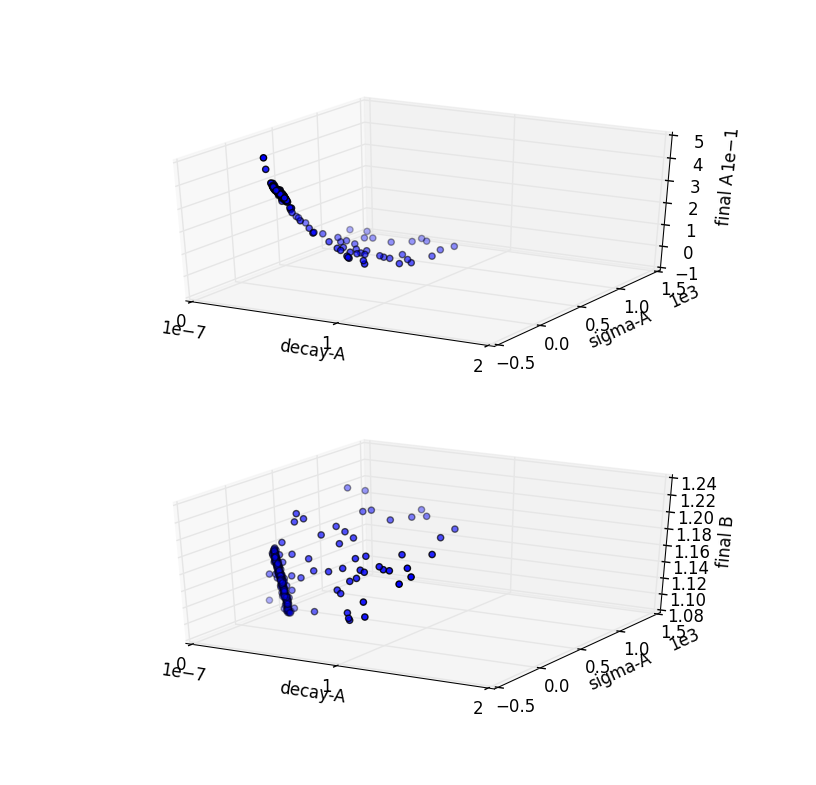
\includegraphics[scale=0.7]{pics/LS_pointsets.png}
  \caption{Plot of the samples generated by the LS search sampling for variables $A,B$.}
  \label{fig:LS_pointsets}
 \end{figure}
 %%%%%%%%%%%%%%%%%%%%%%%%%%%%%%%%%%%%%%%%%%%%%%%%%%%%%%%%%%
 %%%%%%%%%%%%%%%%%%%%%%%%%%%%%%%%%%%%%%%%%%%%%%%%%%%%%%%%%%  
   \item \textbf{\textit{Steps}}:   
\begin{lstlisting}[style=XML,morekeywords={arg,extension,pauseAtEnd,overwrite}]
  <Steps>
    <MultiRun name="sample">
      <Input          class="Files"       type="input">referenceInput.xml</Input>
      <Model          class="Models"      type="Code">testModel</Model>
      <Sampler        class="Samplers"    type="LimitSurfaceSearch">LSsearchSampler</Sampler>
      <SolutionExport class="DataObjects" type="PointSet">limitSurface</SolutionExport>
      <Output         class="DataObjects" type="PointSet">samples</Output>
      <Output         class="DataObjects" type="HistorySet">histories</Output>
    </MultiRun>
    <PostProcess name="computeLSintegral">
      <Input  class="DataObjects" type="PointSet"     >limitSurface</Input>
      <Model  class="Models"      type="PostProcessor">integralLS</Model>
      <Output class="DataObjects" type="PointSet"     >limitSurface</Output>
      <Output class="Files"       type=""             >LSintegral.csv</Output>
    </PostProcess>
    <IOStep name="writeHistories" pauseAtEnd="True">
      <Input  class="DataObjects"      type="HistorySet">histories</Input>
      <Input  class="DataObjects"      type="PointSet">samples</Input>
      <Input  class="DataObjects"      type="PointSet">limitSurface</Input>
      <Output class="OutStreamManager" type="Plot">samplesPlot3D</Output>
      <Output class="OutStreamManager" type="Plot">historyPlot</Output>
      <Output class="OutStreamManager" type="Print">samples</Output>
      <Output class="OutStreamManager" type="Plot">limitSurfacePlot</Output>
      <Output class="OutStreamManager" type="Print">histories</Output>
    </IOStep>
  </Steps>
\end{lstlisting}
  %%%%%%%%%%%%%%%%%%%%%%%%%%%%%%%%%%%%%%%%%%%%%%%%%%%%%%%%%%
 %figure samples
 \begin{figure}[h!]
  \centering
  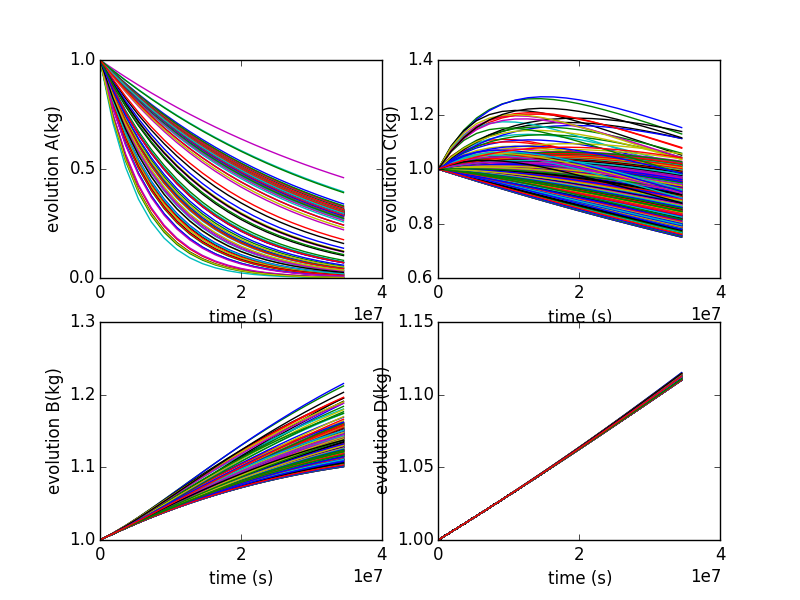
\includegraphics[scale=0.7]{pics/LS_histories.png}
  \caption{Plot of the histories generated by the LS search method for variables $A,B,C,D$.}
  \label{fig:LS_histories}
 \end{figure}
 %%%%%%%%%%%%%%%%%%%%%%%%%%%%%%%%%%%%%%%%%%%%%%%%%%%%%%%%%%
   Finally, all the previously defined \textbf{Entities} can be combined in 
   the \xmlNode{Steps} block. As inferable, 
   3 \xmlNode{Steps} have been inputted:
   \begin{itemize}
     \item \xmlNode{MultiRun} named ``sample'', used to run the multiple  
     instances of the driven code and 
     collect the outputs in the two \textit{DataObjects}. As it can be
     seen, the \xmlNode{Sampler} is inputted to communicate to the 
     \textit{Step} that the driven code needs to
     be perturbed through the LS search sampling strategy;
     \item \xmlNode{PostProcess} named ``computeLSintegral'', used to 
     compute the probability of failure of the system based on the Limit
     Surface generated employing the LS search strategy. This 
     probability is computed integrating the LS with a Monte-Carlo 
     method. 
     \item  \xmlNode{IOStep} named ``writeHistories'', used to 1) dump 
     the ``histories'' and ``samples''  \textit{DataObjects} 
     \textbf{Entity} in a CSV file and 2) plot the data and the Limit Surface 
     in  PNG files and on the screen.
   \end{itemize}
\end{enumerate} 
 Figure~\ref{fig:LS_histories} 
 shows the evolution of the outputs $A,B,C,D$ under uncertainties. 
 Figure~\ref{fig:LS_pointsets} shows the final responses  of $A and B$
 of the sampling employed using the driven code. 
 Figure~\ref{fig:LSplot}  shows the limit surface for this particular 
 example. Only $367$ samples were needed in order to reach the full 
 convergence.
 \\The integration of the LS determines a probability of failure of 
 $~3.45e-2$.
  %%%%%%%%%%%%%%%%%%%%%%%%%%%%%%%%%%%%%%%%%%%%%%%%%%%%%%%%%%
 %figure samples
 \begin{figure}[h!]
  \centering
  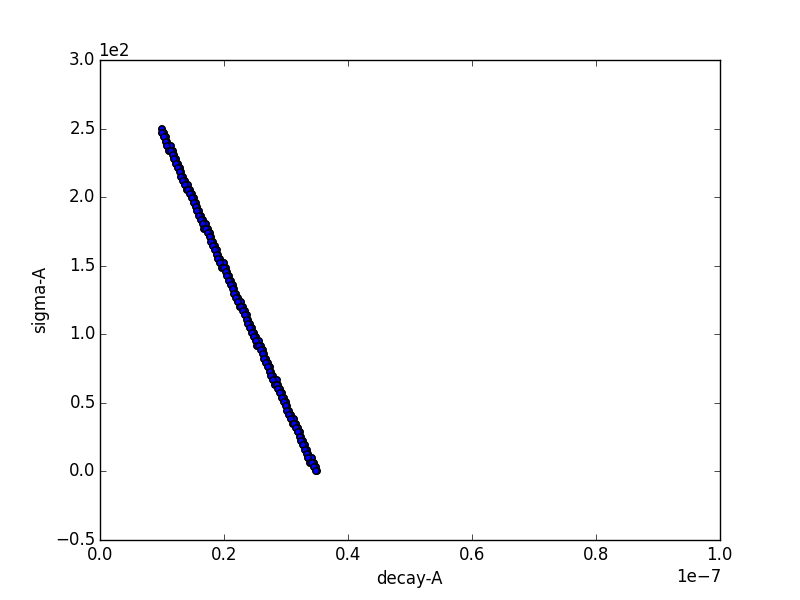
\includegraphics[scale=0.7]{pics/LimitSurfacePlot.png}
  \caption{Limit Surface generated by the LS search method.}
  \label{fig:LSplot}
 \end{figure}
 %%%%%%%%%%%%%%%%%%%%%%%%%%%%%%%%%%%%%%%%%%%%%%%%%%%%%%%%%%








